\documentclass[12pt]{article}

\usepackage{stoversymb,graphicx,soul}
\usepackage[letterpaper, margin=0.5in, top=0.75in, bottom=1in]{geometry}

%\everymath{\displaystyle}

\usepackage{multicol}
\usepackage[many]{tcolorbox}
\usepackage{tikz}

\title{\vspace{-0.75in}\LARGE{Stuff You Need to Know From Calculus}\vspace{-0.5in}}
\date{}

\usepackage[inline]{enumitem}
\setlist[enumerate,1]{leftmargin=0.625in, rightmargin=0.5in, label=(\alph*),itemsep=2.25mm,topsep=1.5mm}
\setlist[enumerate,2]{leftmargin=0.25in}

\newcommand{\shortlim}{\lim_{n\to\infty}}
\newcommand{\sectitle}[1]{\vspace{7.5mm}\noindent\textbf{\Large{#1}}\\[3mm]}
\newcommand{\subsectitle}[2]{\vspace{3mm}\noindent\ul{#1}:\\[3mm]\indent{#2}}
\newcommand{\subsecnoindent}[2]{\vspace{3mm}\noindent\ul{#1}:\\[3mm]{#2}}
\newcommand{\comps}[1]{\langle #1_1,#1_2,#1_3\rangle}
\newcommand{\compslong}[3]{\langle #1, #2, #3\rangle}
\newcommand{\pic}[2]{\begin{center}\includegraphics[scale=#1]{#2}\end{center}}
\newcommand{\resultbox}[1]{\begin{center}
		\begin{tcolorbox}[
			enhanced,
			colback=white,
			colframe=black,
			boxrule=0.5pt,
			arc=0pt,
			top=3mm,
			bottom=3mm, 
			width=7in%,
%			grow to left by=0.5in,
			]
			\centering
			#1
		\end{tcolorbox}
\end{center}}
\newcommand{\LH}{L'H\^{o}pital}

\graphicspath{ {./img/} }
\DeclareGraphicsExtensions{.pdf, .png}

\usepackage{caption}
\captionsetup{labelfont=bf, labelformat=simple, justification=centering, labelsep=newline, width=6.5in, textfont={small}}%, textfont={it, footnotesize}}
\captionsetup[figure]{aboveskip=8pt, belowskip=10pt}

\begin{document}
	\maketitle
	
	\noindent For the first time in the semester, the stuff we're doing is \textit{finally} going to look like calculus (with a vector slant, of course). This means that in order to succeed, you need to remember all that other calculus junk that you've probably forgotten!
	
	Don't fret, though: This review should help you out!
	
	Unless otherwise noted, $f,g,h:\Reals\to\Reals$ will denote real-valued functions on $\Reals$.

	\sectitle{Limits and Continuity}
	Even though most of us can't define it precisely, we all sort of \textit{know} what it means to ``take the limit'' of the values of a function $f$, say, as $x$ approaches $a$: It means we analyze the values of $f(x)$ as $x$ ``gets close to'' $a$, and most of the time, we accomplish this either by (a) plugging $x=a$ into $f$ directly, or (b) doing algebra on $f$ (e.g. factoring,...) until we \textit{can} plug in $x=a$. 
	
	We may not always get a value this way, but if we \textit{do} get a value (say, $L$), we write
	$$\lim_{x\to a}f(x)=L$$
	for the value of the limit. As it happens, this approach almost always works for elementary stuff, and later (read: \textit{after we know derivatives}), we have additional tools such as \LH's rule to help us evaluate even more limits.
	
	That's fine and good, and in Calc 3, we'll almost always use the techniques we already have to evaluate higher-dimensional analogues of this concept. Even so, here's the \textit{real} definition of a limit, just so you can say you've seen it before.\vspace{6mm}
		
	\noindent\textbf{Definition:} The real number $L$ is said to be the \textit{limit of the function $f$ as $x\to a$} if
	\begin{equation}
		\label{eq:limdef}
		\text{for all }\eps>0\text{, there exists a }\delta>0\text{ such that }|f(x)-L|<\eps\text{ whenever }|x-a|<\delta.
	\end{equation}
	In this case, we write $L=\lim_{x\to a}f(x)$.\vspace{3mm}
	
	\begin{figure}[h!]
		\centering
		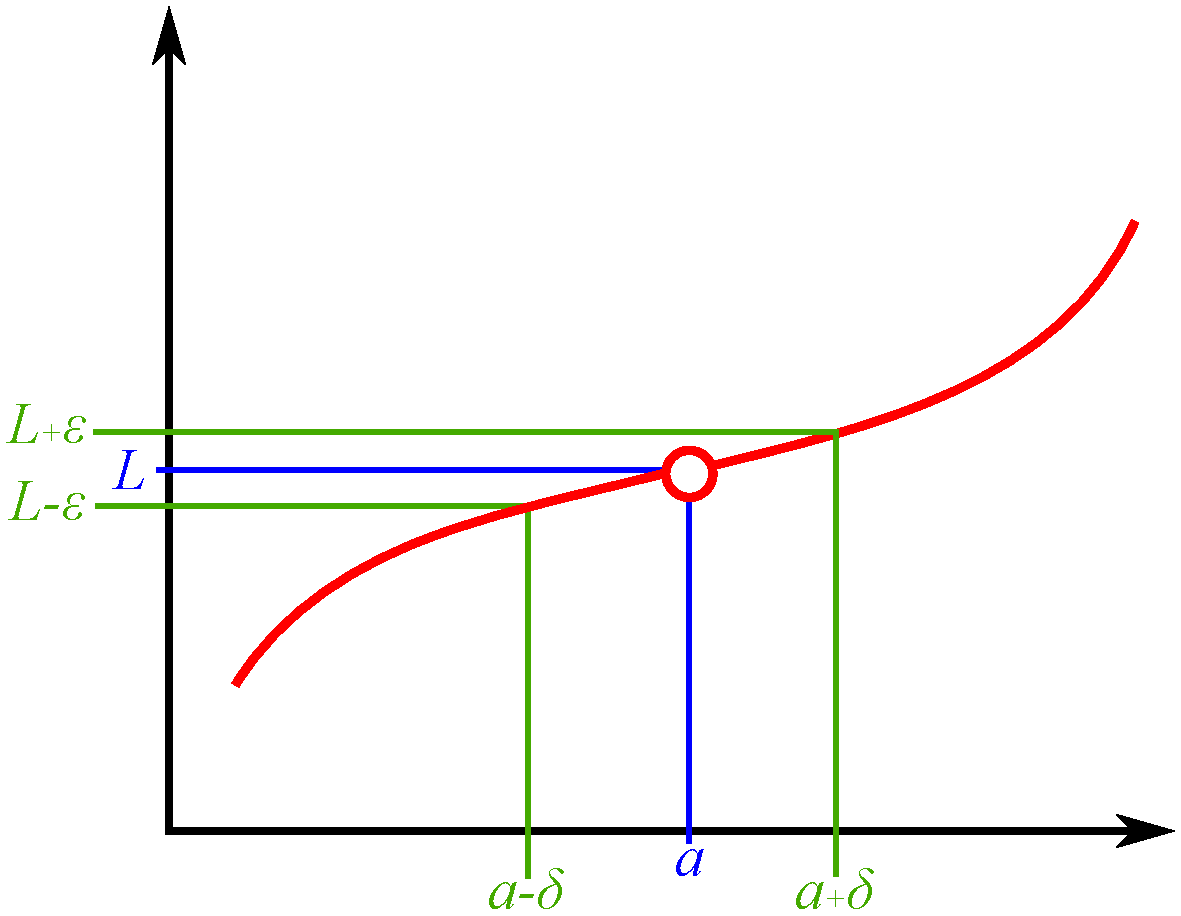
\includegraphics[width=3.5in]{limit}
		\caption{Even though $f(a)\neq L$, the limit $\lim_{x\to a}f(x)$ \textit{does} equal $L$ because for \ul{every} $\eps>0$ (no matter how small), there is an interval $(x-\delta,x+\delta)$ on the \textbf{$\boldsymbol{x}$-axis} which maps to the interval $(L-\eps,L+\eps)$ on the \textbf{$\boldsymbol{y}$-axis}. Note that smaller $\eps$ values (i.e. smaller intervals on the $y$-axis) will require smaller $\delta$ values (i.e. smaller intervals on the $x$-axis).}
		\label{fig:limit}
	\end{figure}
	
	The condition in \eqref{eq:limdef} is esoteric to be certain, but as the figure \ref{fig:limit} shows, it properly characterizes the notion most of us have in our minds.
	
	Recall that we \textit{also} have notions of ``limits from the left / below'' and ``limits from the right / above'' which we shouldn't forget. Without beating a dead horse, you should recall what these ``one-sided limits'' mean, intuitively, and you should always remember that \ul{$L$ is the limit of $f$ as $x\to a$ in the sense of {\eqref{eq:limdef}} if and only if $L$ is the limit from the left \textit{and} from the right}:
	$$\lim_{x\to a}f(x)=L\text{ if and only if}\lim_{x\to a^-}f(x)=L\text{ \ul{\textbf{and}} }\lim_{x\to a^+}f(x)=L.$$
	
	As it happens, limits distribute over sums, differences, scalar multiplication, division, and powers; in addition, common results such as the squeeze theorem also hold.
	
	In short: Limits provide the framework needed to allow us the privilege of talking about the values of functions close to ``bad spots'' like holes, jumps, and vertical asymptotes in ways that we couldn't do in algebra, for example. 
	
	Of course, not all functions \textit{have} ``bad spots'' like holes, jumps, and vertical asymptotes, and as a way to differentiate those from the rest, we have a special word.\vspace{6mm}
	
	\noindent\textbf{Definition:} The function $f:\Reals\to\Reals$ is said to be \textit{continuous at $x=a$} if:
	\begin{enumerate}
		\item $f(a)$ exists (as a real number);
		\item $\lim_{x\to a}f(x)$ exists (as a real number); and
		\item $\lim_{x\to a}f(x)=f(a)$.
	\end{enumerate}\vspace{3mm}

	Intuitively, we imagine that a function is continuous if and only if we're able to draw the entirety of its graph without having to lift our pencil (so that it has no holes, no jumps, no vertical asymptotes...), and as figure \ref{fig:discont} shows, each of these conditions is necessary for our definition to match our intuition.
	
	\begin{figure}[h!]
		\centering
		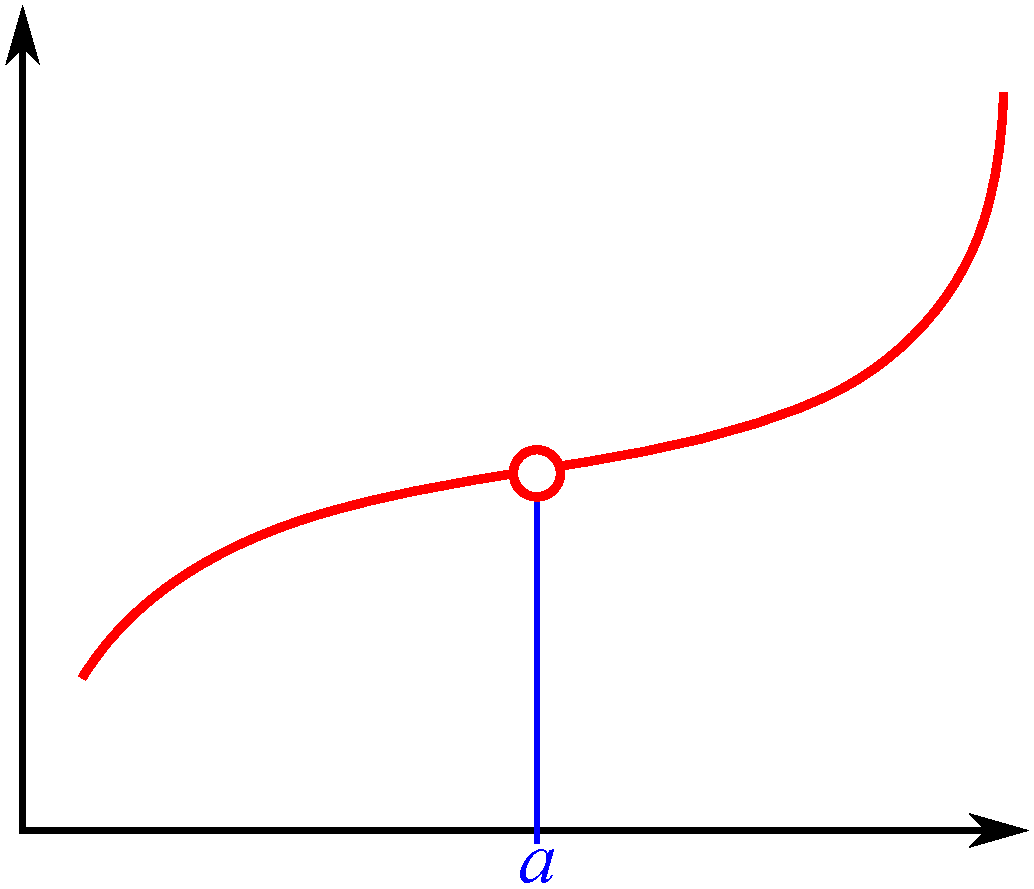
\includegraphics[width=2.125in]{discont1}
		\quad
		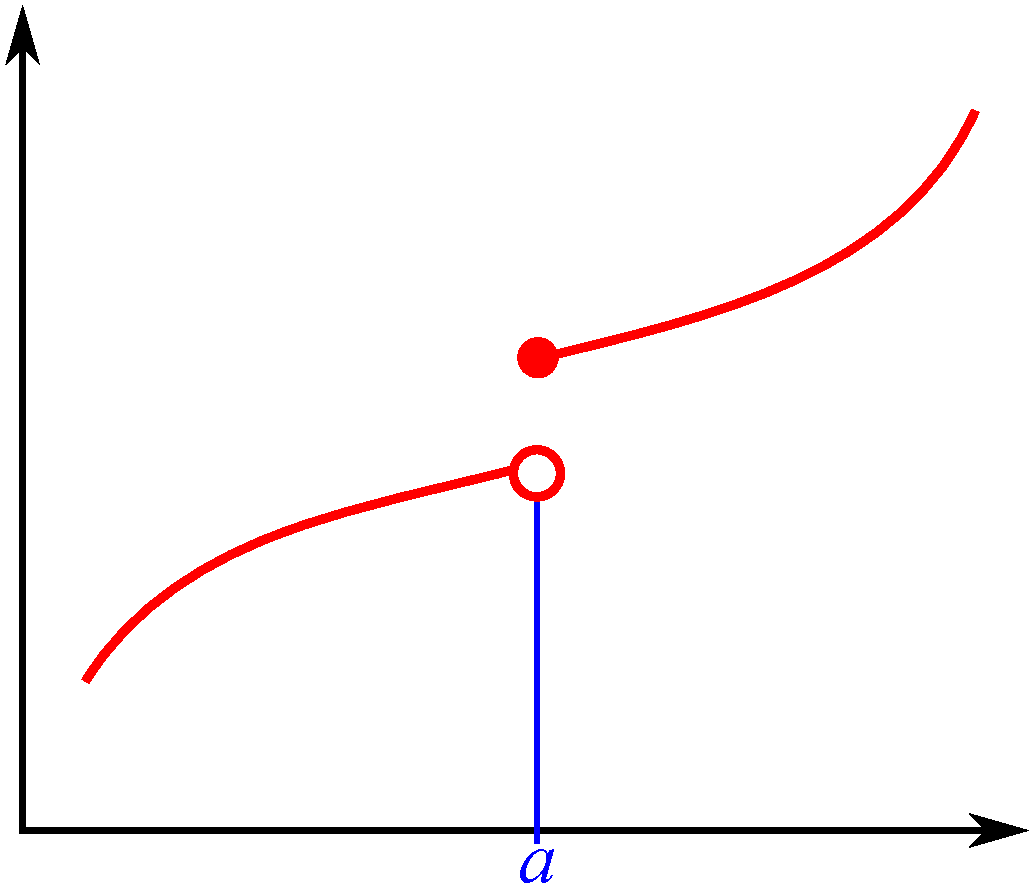
\includegraphics[width=2.125in]{discont2}
		\quad
		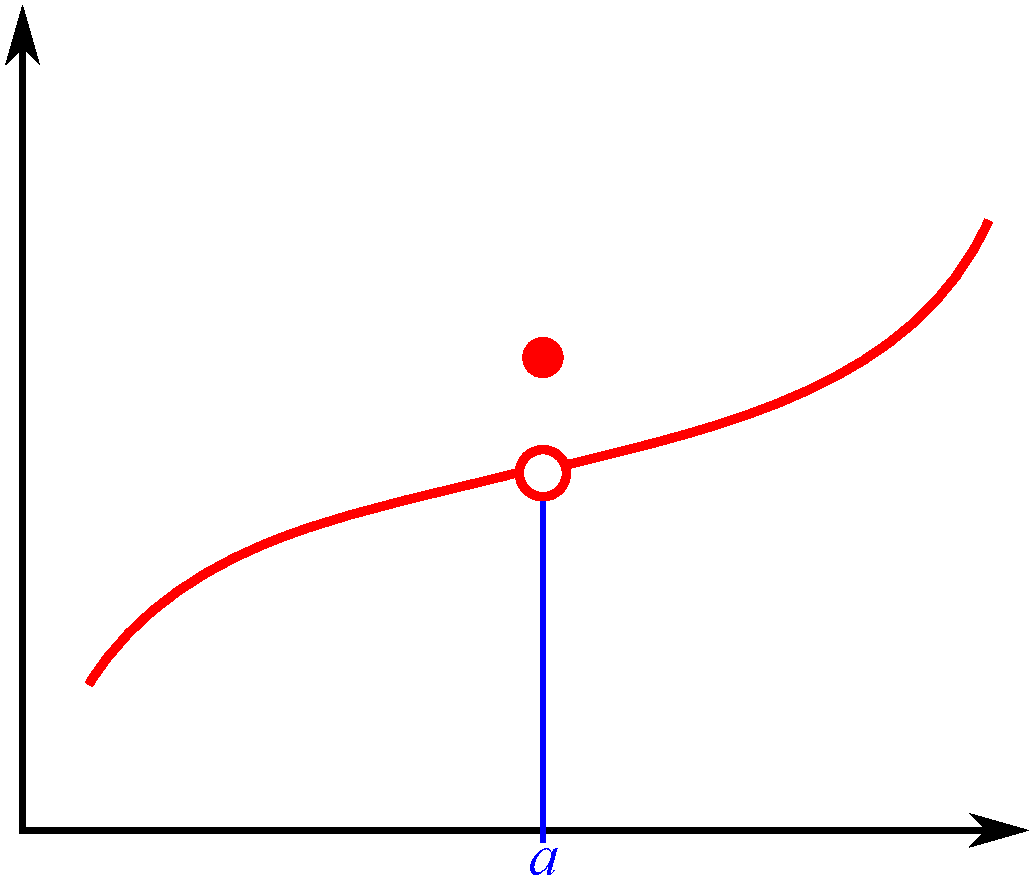
\includegraphics[width=2.125in]{discont3}
		\caption{Discontinuity may mean violating any of the three above conditions: $f(a)$ may fail to exist (left), $\lim_{x\to a}f(x)$ may fail to exist (middle), or both may exist and satisfy $\lim_{x\to a}f(x)\neq f(a)$ (right).}
		\label{fig:discont}
	\end{figure}

	Taking limits of continuous functions is easier overall because of property (c): To take the limit as $x\to a$ of a function which is continuous at $x=a$, it suffices to ``just plug in'' $a$. In addition, if $f$ and $g$ are defined and continuous at the point $x=a$ and if $c$ is any constant, the functions $f\pm g$, $fg$, $f/g$ (if $g(a)\neq 0$), $cf$, $f\circ g$, and $g\circ f$ are all continuous at $x=a$ (assuming the compositions meet the appropriate domain/range restrictions). Significant results such as the intermediate value theorem also hold.

	\sectitle{Derivatives \& Differentiability}
	First, the definitions.\vspace{6mm}
	
	\noindent\textbf{Definition:} The \textit{derivative of a function $f$ at $x=a$} (if it exists) is the number
	\begin{equation}
		\label{eq:der}
		f'(a)=\lim_{h\to 0}\frac{f(a+h)-f(a)}{h}.
	\end{equation}
	In this case, we say that $f$ is \textit{differentiable at $x=a$}.\vspace{3mm}
	
	\vspace{6mm}
	
	\noindent\textbf{Definition:} The \textit{derivative of a function $f$} (if it exists) is the function $f'(x)$ defined by
	\begin{equation}
		\label{eq:der2}
		f'(x)=\lim_{h\to 0}\frac{f(x+h)-f(x)}{h}.
	\end{equation}
%	In this case, we say that $f$ is \textit{differentiable at $x=a$}.\vspace{3mm}

	Of course, equations \eqref{eq:der} and \eqref{eq:der2} have all the quantitative and qualitative properties we know and love from Calc 1: $f'(a)$ in \eqref{eq:der} describes the slope of the tangent line to the curve $y=f(x)$ at $x=a$, for example, and if $r(x)$ is a differentiable function describing the position of a particle (or whatever), the functions $v(x)=r'(x)$ and $a(x)=v'(x)=r''(x)$ describe the velocity and acceleration of the particle, respectively.
	
	As we know from Calc 1, not all functions have derivatives: In particular, a function which fails to be continuous at $x=a$ will clearly not have a derivative there, though some continuous functions may \textit{also} not be differentiable everywhere (e.g. $f(x)=|x|$ fails to have a derivative at $x=0$). 
	
	In this way, being differentiable is \textit{stronger} than being continuous, and in general, we expect a function $f$ to be differentiable at a point $x=a$ if $f$ is continuous at $a$ \textit{and} if the graph $y=f(x)$ has no ``sharp corners'' and/or vertical tangents at $x=a$. Said differently: If $f$ is differentiable at $x=a$, then when we zoom in toward the point $(a,f(a))$, the graph straightens out and appears more and more like a line. Figure \ref{fig:nodiff} illustrates this.
	
	\begin{figure}[ht!]
		\centering
		\includegraphics[width=7in]{nodiff}
		\caption{The function on the left is differentiable at $x=a$, as zooming in closer and closer to $(a,f(a))$ reveals that the graph becomes more and more linear; the function on the right \textit{isn't}, because no matter how much you zoom in, it always has a point.}
		\label{fig:nodiff}
	\end{figure}
	
	By now, we're all pros at derivatives: We know that derivatives distribute over addition/subtraction and scalar multiplication, and we know that we can use the product rule, the quotient rule, and the chain rule to compute derivatives of products, quotients, and compositions, respectively. Even so, however, we shouldn't forget how to compute $f'(x)$ using equation \eqref{eq:der2}, as that will sometimes be required.


	\subsectitle{Other Uses for Derivatives, Briefly}
	{
		You shouldn't forget the ``extras'' that you're able to do with derivatives, as many of these will also come up in vector-valued functions. Some examples:
	}
	\begin{itemize}
		\item Linear approximations
		\item Implicit/logarithmic differentiation
		\item Related rates (ugh!) \& optimization
		\item \LH's rule for finding limits involving indeterminate forms (many of which arise when investigating information about horizontal asymptotes, etc.)
		\item Mean value theorem (!!!)
		\item Information about where functions are increasing/decreasing, concave up/down, etc.
	\end{itemize}

	\noindent Suffice it to say: If you're even a little bit rusty at derivatives, you need to get unrusty \textit{yesterday}.
	
	\sectitle{Antiderivatives \& Integrability}
	We all (mostly) know the spiel:\vspace{6mm}
	
	\noindent\textbf{Definition:} The \textit{antiderivative of a function $f$} (if it exists) is a function $F$ for which
	\begin{equation}
		\label{eq:antider}
		F'(x)=f(x)
	\end{equation}
	As it happens, every function which is continuous on an interval $[a,b]$ has an antiderivative on the same interval.
	
	By the first part of the fundamental theorem of calculus,
	\begin{equation}
		\label{eq:ftc1}
		F(x)\deff\int_a^xf(t)\,dt
	\end{equation}
	is one such antiderivative of $f$ on the interval $[a,b]$ (where we let $x$ vary between $a$ and $b$), and as we find out later, \textit{every} antiderivative $G$ of $f$ is just a vertical translate of \eqref{eq:ftc1}:
	$$G(x)\text{ is an antiderivative of }f(x)\text{ if and only if }G(x)=C+\int_a^xf(t)\,dt\text{ for some }C.$$
	One can easily show that such a $G$ satisfies \eqref{eq:antider}, and using the fact that $G'(x)=f(x)=F'(x)$, it follows that $G(x)-F(x)$ is a constant (see Corollary 7 in section 3.2 of Stewart). The result follows immediately.
	
	In two-dimensions, the \textit{definite} integral $\int_a^b f(x)\,dx$ gives the (signed) area of the region bounded by $f(x)$ and the $x$-axis from $x=a$ to $x=b$. Recall that the definite integral is defined as the limit of Riemann sums, and by the second part of the fundamental theorem of calculus,
	$$\int_a^b f(x)\,dx=F(b)-F(a)$$
	where $F$ is \ul{any} antiderivative of $f$. This shows in particular that finding  antiderivatives/indefinite integrals is essentially the same as finding definite integrals.
	
	One of the most important properties of antiderivatives is that they're inverses of derivatives:
	$$\frac{d}{dx}\left(\int_a^x f(t)\,dt\right)=f(x)\quad\text{and}\quad \int_a^xf'(t)\,dt=f(x)-f(a).$$
	Intuitively, this means that integrals ``cancel'' derivatives and vice versa. It also means that we can ``go backwards'' in applications: For example, the position $r(x)$, velocity $v(x)$, and acceleration $a(x)$ of a particle (or whatever) is \textit{also} related by the equations $r(x)=C_1+\int v(x)\,dx$ and $v(x)=C_2+\int a(x)\,dx$.
	
	As we learned in Calc 2, integrals \textit{also} have lots of applications to arc length, surface area, etc.; for the sake of brevity, that won't be discussed here, but it \textit{should} be noted that those things \textit{will} come up (sooner than later) in Calc 3.
	
	\sectitle{Formulas you \textit{have} to know!}
	Here is a brief summary of formulas you'll have to know to succeed in this course.
	
	\subsecnoindent{Limits}
	{
		 If $c$ is a constant and the limits $\lim_{x\to a}f(x)$ and $\lim_{x\to a}g(x)$ both exist, then:
		\begin{itemize}[leftmargin=0.375in,itemsep=0.1875in,label=$\circ$]
			\item $\lim_{x\to a}\left[f(x)\pm g(x)\right]=\lim_{x\to a}f(x)\pm\lim_{x\to a}g(x)$
			\item $\lim_{x\to a}\left[c f(x)\right]=c \lim_{x\to a}f(x)$
			\item $\lim_{x\to a}\left[f(x) g(x)\right]=\lim_{x\to a}f(x)\cdot\lim_{x\to a}g(x)$
			\item $\displaystyle\lim_{x\to a}\frac{f(x)}{g(x)}=\frac{\lim_{x\to a}f(x)}{\lim_{x\to a}g(x)}$
			\item $\lim_{x\to a}\left[f(x)\right]^n=\left[\lim_{x\to a}f(x)\right]^n$
			\item (Squeeze theorem) If $f(x)\leq g(x)\leq h(x)$ when $x$ is near $a$ and if $\lim_{x\to a}f(x)=L=\lim_{x\to a}h(x)$, then
			$$\lim_{x\to a}g(x)=L.$$
		\end{itemize}
	}
	\newpage
	\subsecnoindent{Derivatives}
	{
		If $c$ is a constant and if $f$ and $g$ are both differentiable, then:
		\begin{multicols}{2}
		\begin{itemize}[leftmargin=0.375in,itemsep=0.0625in,label=$\circ$]
			\item $\displaystyle\frac{d}{dx}(c)=0$
			\item $\displaystyle\frac{d}{dx}\left(x^n\right)=nx^{n-1}$
			\item $(cf)'=cf'$
			\item $(f\pm g)'=f'\pm g'$
			\item $(fg)'=fg'+f'g$
			\item $\displaystyle\left(\frac{f}{g}\right)'=\frac{f'g-fg'}{g^2}$
			\item $\displaystyle\frac{d}{dx}\left(f(g(x))\right)=f'(g(x))\cdot g'(x)$
		\end{itemize}
		\end{multicols}
	
		\noindent Also:
		\begin{multicols}{3}
			\begin{itemize}[leftmargin=0.375in,itemsep=0.0625in,label=$\circ$]
				\item $\displaystyle\frac{d}{dx}(\sin{x})=\cos{x}$
				\item $\displaystyle\frac{d}{dx}(\cos{x})=-\sin{x}$
				\item $\displaystyle\frac{d}{dx}(\tan{x})=\sec^2{x}$
				\item $\displaystyle\frac{d}{dx}(\csc{x})=-\csc{x}\cot{x}$
				\item $\displaystyle\frac{d}{dx}(\sec{x})=\sec{x}\tan{x}$
				\item $\displaystyle\frac{d}{dx}(\cot{x})=-\csc^2{x}$
				\item $\displaystyle\frac{d}{dx}(\sin^{-1}(x))=\frac{1}{\sqrt{1-x^2}}$
				\item $\displaystyle\frac{d}{dx}(\cos^{-1}(x))=-\frac{1}{\sqrt{1-x^2}}$
				\item $\displaystyle\frac{d}{dx}(\tan^{-1}(x))=\frac{1}{1+x^2}$
%				\item $\displaystyle\frac{d}{dx}(\csc^{-1}(x))=-\csc{x}\cot{x}$
%				\item $\displaystyle\frac{d}{dx}(\sec^{-1}(x))=\sec{x}\tan{x}$
%				\item $\displaystyle\frac{d}{dx}(\cot^{-1}(x))=-\csc^2{x}$ 
				\columnbreak
				\item $\displaystyle\frac{d}{dx}(a^x)=a^x\ln{a}$
				\item $\displaystyle\frac{d}{dx}(e^x)=e^x$ 
				\item $\displaystyle\frac{d}{dx}(\ln{x})=\frac{1}{x}$
				\item $\displaystyle\frac{d}{dx}(\log_b{x})=\frac{1}{x\ln{b}}$
			\end{itemize}
		\end{multicols}
	}
	\subsecnoindent{Integrals}
	{
		You should \textbf{definitely} know how to ``go backwards'' on the list of derivatives to rewrite in terms of integrals: For example, 
		$$\displaystyle\frac{d}{dx}(\tan^{-1}(x))=\frac{1}{1+x^2}\Longleftrightarrow\int\frac{1}{1+x^2}\,dx=\tan^{-1}(x)+C.$$
		You \textit{also} need to now how to do $u$-substitution, integration by parts, trig substitution, and integration by partial fractions, as well as how to integrate products of powers of trig functions (e.g. $\int\sin^2{x}\cos^3{x}\,dx$).\vspace{3mm}
		
		\noindent In addition: If $k$ is a constant and if $f$ and $g$ are both integrable, then:
		\begin{multicols}{2}
			\begin{itemize}[leftmargin=0.375in,itemsep=0.0625in,label=$\circ$]
				\item $\int k\,dx=kx + C$
				\item $\int x^n\,dx=\frac{x^{n+1}}{n+1}+C$
				\item $\int kf\,dx=k\int f(x)\,dx + C$
				\item $\int (f\pm g)\,dx=\int f\,dx\pm \int g\,dx + C$
%				\item $(fg)'=fg'+f'g$
%				\item $\displaystyle\left(\frac{f}{g}\right)'=\frac{f'g-fg'}{g^2}$
%				\item $\displaystyle\frac{d}{dx}\left(f(g(x))\right)=f'(g(x))\cdot g'(x)$
			\end{itemize}
		\end{multicols}
		
		\noindent Finally:
		\begin{multicols}{2}
			\begin{itemize}[leftmargin=0.375in,itemsep=0.0625in,label=$\circ$]
				\item $\int \ln{x}\,dx=x\ln{x}-x+C$
				\item $\int \tan{x}\,dx=\ln|\sec{x}|+C$
				\item $\int \cot{x}\,dx=\ln|\sin{x}|+C$
				\item $\int \sec{x}\,dx=\ln|\sec{x}+\tan{x}|+C$
				\item $\int \csc{x}\,dx=\ln|\csc{x}-\cot{x}|+C$
			\end{itemize}
		\end{multicols}
	}
\end{document}